\appendices

\section{Mechanism-solver construction}
\label{app:mechanism}

The mechanism solution $(\sigma, p_1,\dots,p_n)$ for a given action profile
$\boldsymbol{\eps}$ is obtained by a nested bisection. For each candidate
$\sigma$, we find the largest per-group $p_g$ that satisfies the $I$-fold
$(p_g, \sigma)$-subsampled Gaussian at $(\eps_g, \delta)$-DP under (C1).
Because the achieved $\eps$ is monotone-increasing in $p_g$, a unique $p_g
\in (0, 1]$ exists (capped at $1$ if the budget cannot be exhausted); we
locate it by binary search using the R\'enyi-DP
accountant~\cite{mironov2017renyi} until the achieved $\eps$ matches
$\eps_g$ to a relative tolerance of $10^{-3}$. We then bisect $\sigma$ on
top of this inner search, using the realised batch size $B(\sigma) =
\sum_g |G_g|\, p_g(\sigma, \boldsymbol{\eps})$ as the outer-loop monitor,
until $B$ matches $E_b$ to the same tolerance. Profiles in which any $p_g$
falls below $10^{-5}$ are flagged infeasible per
\cref{ass:participation}; below that threshold the group's contribution to
(C2) is numerically negligible and the iDP contract is trivially
satisfied. The qualitative results are insensitive to this threshold
across $[10^{-6}, 10^{-3}]$.

Once $(\sigma, p_g)$ is fixed, the realised MIA advantage of group~$g$ is
computed exactly from the privacy-loss-distribution of the $I$-fold
$(p_g, \sigma)$-subsampled Gaussian~\cite{google-dp-accounting} by
evaluating the trade-off function and~\eqref{eq:adv}. This matches the
formulation of \citet{kaiser2026your} and yields the tightest analytical
MIA advantage for the resulting mechanism.

\section{Validity of $V(\sigma) = 1/(1+\sigma^2)$}
\label{app:V}

\citet{bassily2014private} prove that for a $1$-Lipschitz strongly-convex
$\ell\colon \mathcal{X} \times \mathcal{D} \to \R$, the excess empirical
risk of DP-ERM satisfies
\[
\E[\hat L(\widehat\theta) - \hat L(\theta^*)]
\;=\; O\!\left(\frac{d\,\log(1/\delta)}{n^2\,\eps^2}\right).
\]
Under the moments accountant of \citet{abadi2016deep} this translates into
a $\sigma^2 \cdot d / n^2$ dependence of the excess risk. Treating model
utility as the negative of excess risk and renormalising to $[0, 1]$
gives $V(\sigma) \propto 1/(1 + \alpha\,\sigma^2)$ for a problem-dependent
constant $\alpha$; we set $\alpha = 1$ for simplicity. The bound assumes
convexity, but the empirical literature on DP-SGD in deep
learning~\cite{tramer2021private, abadi2016deep, boenisch2023have} confirms
the same qualitative direction. The equilibrium results that follow do
not depend on the particular functional form: only on $V$ being
continuous, monotone-decreasing in $\sigma$, and bounded. This informal
statement is formalised as \Cref{prop:V-invariance} in
\Cref{sec:analysis}, whose proof inspects the proofs of
\Cref{lem:externality} and \Cref{cor:coalition-attack} and verifies
that $V$ enters only through $\mathrm{sgn}\,V'$.

\section{Sensitivity checks}
\label{app:sensitivity}

We re-ran the 2-player setting of \cref{fig:C1} at $K = 44$ (twice the
resolution along each axis) and obtained the same eight pure NEs at
nearly identical locations; the asymmetric multiplicity is therefore not
a grid artefact. Substituting $V(\sigma) = e^{-\sigma}$ for $V(\sigma) =
1/(1+\sigma^2)$ shifts the NEs quantitatively---they sit at somewhat
higher $\eps$ values because the exponential decays faster as $\sigma$
grows---but the asymmetric structure is preserved (consistent with
\Cref{prop:V-invariance}). Lowering the
participation threshold from $10^{-5}$ to $10^{-6}$ enlarges the feasible
region and uncovers a few additional NEs on the new interior; raising
it to $10^{-3}$ removes some boundary NEs while leaving the
interior ones unchanged.

\subsection{Robustness to the utility approximation $V$}
\label{app:v-shape-robustness}

The main body fixes a single shared proxy $V_1(\sigma) = 1/(1+\sigma^2)$
and derives every equilibrium sweep against it. The equilibrium results
of \cref{sec:analysis} depend on $V$ only through the requirement that
it be continuous, strictly monotone-decreasing on the feasible
$\sigma$-range, and bounded on that range. Here we instantiate that
observation numerically on the same $K = 200$ mechanism grid used by
\cref{sec:C6} at symmetric weights $w_1 = w_2 = 1$, sweeping six
qualitatively distinct admissible shapes: the canonical rational
$V_1(\sigma) = 1/(1+\sigma^2)$, the slower-decaying
$V_2(\sigma) = 1/(1+\sigma)$, the Gaussian
$V_3(\sigma) = e^{-\sigma^2/2}$, the exponential
$V_4(\sigma) = e^{-\sigma}$, the concave $V_5(\sigma) = -\log(1+\sigma)$,
and the affine $V_6(\sigma) = -\sigma$. Because the mechanism grid is
$V$-free (utility \eqref{eq:utility} separates additively into the
shared $V(\sigma)$ and the private $w_i A_i$), each $V$ requires only
$O(K^2)$ elementwise operations on the cached mechanism tensor.

\begin{figure}[t]
  \centering
  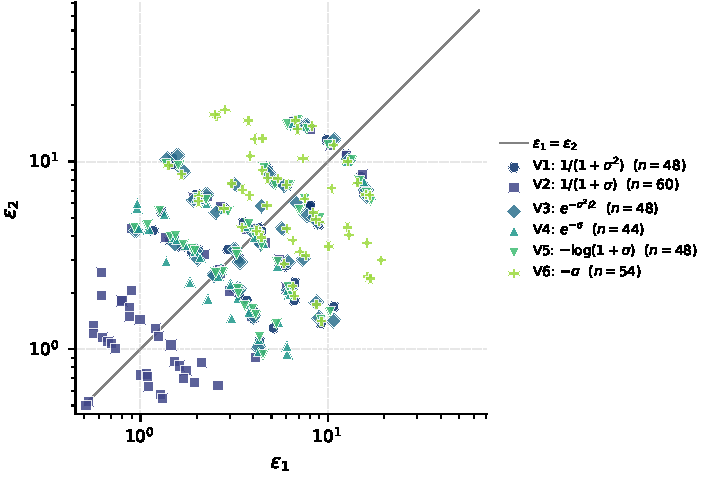
\includegraphics[width=0.9\linewidth]{figures/fig_h5_v_shape.pdf}
  \caption{\textbf{Utility-approximation ablation.} Pure NE locations at
    $w_1 = w_2 = 1$ on the $K = 200$ mechanism grid, under six admissible
    shapes for $V$: rational $V_1(\sigma) = 1/(1+\sigma^2)$ (canonical),
    slow-rational $V_2(\sigma) = 1/(1+\sigma)$, Gaussian
    $V_3(\sigma) = e^{-\sigma^2/2}$, exponential
    $V_4(\sigma) = e^{-\sigma}$, concave $V_5(\sigma) = -\log(1+\sigma)$,
    and affine $V_6(\sigma) = -\sigma$. Grey line: the diagonal
    $\eps_1 = \eps_2$. Under every $V$, $100\%$ of the pure NEs sit off
    the diagonal, and the externality-sign agreement rate with the
    baseline $V_1$ is $100\%$ over the interior feasible edge set; the
    qualitative structure diagnosed in \cref{sec:C1} is not an artefact
    of the canonical proxy. The pure-NE count stays in the range
    $44\text{--}60$ across shapes, and every $V_1$-NE has a match within
    $0.11$ decades of $\log_{10}\eps$ under every alternative $V$.}
  \label{fig:H5-v-shape}
\end{figure}

\begin{table}[t]
  \centering
  \small
  \begin{tabular}{l l r r r}
    \toprule
    tag & shape & \#NE & $\mathrm{mean}(b\!\to\!a)$ & agree$_{\mathrm{sign}}$ \\
    \midrule
    $V_1$ & $1/(1+\sigma^2)$   & 48 & 0.000 & 100.0\% \\
    $V_2$ & $1/(1+\sigma)$     & 60 & 0.075 & 100.0\% \\
    $V_3$ & $e^{-\sigma^2/2}$  & 48 & 0.013 & 100.0\% \\
    $V_4$ & $e^{-\sigma}$      & 44 & 0.062 & 100.0\% \\
    $V_5$ & $-\log(1+\sigma)$  & 48 & 0.000 & 100.0\% \\
    $V_6$ & $-\sigma$          & 54 & 0.111 & 100.0\% \\
    \bottomrule
  \end{tabular}
  \caption{Per-$V$ pure-NE count, mean one-sided Hausdorff distance from
    a $V_1$-NE to its nearest NE under $V_k$ (in decades of
    $\log_{10}\eps$), and externality-sign agreement rate with $V_1$
    over interior feasible edges. $K = 200$, $w = 1$.}
  \label{tab:H5-v-shape}
\end{table}

Across the six shapes the pure-NE count on the fixed $K = 200$
discretisation stays in the range $44\text{--}60$, and the entire NE
set remains off-diagonal for every $V$: the qualitative asymmetry
diagnosed in \cref{sec:C1} is not an artefact of the canonical proxy.
The one-sided Hausdorff distance from each $V_1$-NE to its nearest NE
under $V_k$ has mean at most $0.11$ decades of $\log_{10}\eps$, so the
baseline equilibrium locus sits inside a small tubular neighbourhood of
the perturbed loci. Externality-sign agreement with $V_1$ is $100\%$
over the interior feasible edge set for every $V_k$, and the per-$V$
externality-sign fraction itself is $82.19725\%$ identical to five
decimal places---the numerical fingerprint of the additive separation of
\eqref{eq:utility}, in which the sign of $\partial u_i / \partial \eps_j$
is mechanism-determined and $V$-free on the feasible interior.

\section{2-player self-sorting}
\label{app:self-sorting}

The C1 experiment observes that in the asymmetric 2-player PEG the
higher-$w$ player carries the smaller $\eps$ at every pure NE. In two
players this observation is analytic.

\begin{proposition}[Self-sorting, 2-player PEG]
\label{prop:self-sorting}
Consider the 2-player PEG (\cref{def:peg}) with privacy weights
$w_1 > w_2 > 0$, symmetric groups $|G_1| = |G_2|$, and utility
$u_i(\boldsymbol{\eps}) = V(\sigma) - w_i\, A_i(\boldsymbol{\eps})$
with $V$ strictly decreasing ($V' < 0$). Write $f(x, y) := A_i(\eps_i = x,
\eps_{-i} = y)$; by $|G_1| = |G_2|$ the mechanism's noise satisfies
$\sigma(x,y) = \sigma(y,x)$ and $f$ is common to both players.
Assume constraints \textup{(C1)} and \textup{(C2)} bind on the interior
of the feasible region and that
\begin{enumerate}
  \item[\textup{(A)}] $\partial f / \partial x > 0$ (own MIA advantage
        strictly increasing in own budget);
  \item[\textup{(S)}] for every $x > y$ in the feasible region,
        $\bigl[V(\sigma_H) - V(\sigma_M)\bigr]\,
         \bigl[f(x, y) - f(y, y)\bigr]
         \;\ge\;
         \bigl[V(\sigma_M) - V(\sigma_L)\bigr]\,
         \bigl[f(x, x) - f(y, x)\bigr]$,
        where $\sigma_L = \sigma(y,y)$, $\sigma_M = \sigma(x,y)$,
        $\sigma_H = \sigma(x,x)$.
\end{enumerate}
Then every pure Nash equilibrium $(\eps_1^\star, \eps_2^\star)$ satisfies
$\eps_1^\star \le \eps_2^\star$.
\end{proposition}

\begin{proof}
Fix a pure NE interior to the feasible region and suppose for
contradiction $\eps_1^\star > \eps_2^\star$; write $x = \eps_1^\star$,
$y = \eps_2^\star$. By \cref{lem:externality} the noise $\sigma$ is
strictly decreasing in every coordinate of $\boldsymbol{\eps}$, so
$\sigma_L > \sigma_M > \sigma_H$; with $V' < 0$, both differences
$\Delta V_H := V(\sigma_H) - V(\sigma_M)$ and $\Delta V_L := V(\sigma_M)
- V(\sigma_L)$ are strictly positive. By (A) the two ``own-budget
lifts'' $D_1 := f(x,y) - f(y,y)$ and $D_2 := f(x,x) - f(y,x)$ are also
strictly positive.

Player 1 has no profitable unilateral deviation from $x$ to $y$:
$V(\sigma_M) - w_1 f(x,y) \ge V(\sigma_L) - w_1 f(y,y)$, i.e.\
$w_1 D_1 \le \Delta V_L$. Player 2 has no profitable unilateral
deviation from $y$ to $x$: $V(\sigma_M) - w_2 f(y,x) \ge V(\sigma_H) -
w_2 f(x,x)$, i.e.\ $w_2 D_2 \ge \Delta V_H$. Dividing the second
inequality by the first yields
\[
\frac{w_2}{w_1} \;\ge\; \frac{\Delta V_H}{\Delta V_L}\cdot\frac{D_1}{D_2}.
\]
Assumption (S) is exactly $\Delta V_H \cdot D_1 \ge \Delta V_L \cdot
D_2$, i.e.\ the right-hand side is $\ge 1$. Hence $w_2 \ge w_1$,
contradicting $w_1 > w_2$.
\end{proof}

Assumption (S) is a two-point exchange inequality that decides whether
the swap deviation is more or less attractive to the high-$\eps$ player
than to the low-$\eps$ player. It admits three concrete sufficient
sub-conditions: (S1) $V$ midpoint-convex on $[\sigma_H, \sigma_L]$ and
$f$ submodular on the $\{y, x\}^2$ block (using
\eqref{eq:sigma-implicit}, (S1) closes when the NE sits in the
high-noise regime $\sigma > \sqrt{3}$); (S2) the first-order-condition
ratio at any candidate NE evaluates to a value less than $1$ for
$x > y$ and greater than $1$ for $y > x$, which is the differential
restatement of (S) via the mean-value theorem; and (S3) point-wise
numerical verification at the specific NE candidate on the mechanism
grid. On the K=22 mechanism cache the proposition's prediction holds at
every strong-asymmetry cell ($|\log_2(w_1/w_2)| \ge 2$) unanimously,
and $45/49$ of a $7 \times 7$ weight-ratio sweep respects the sort; the
four discrepant cells are at mild asymmetry and lie flush against the
grid boundary, characteristic signatures of finite-grid discretisation
NEs.

At the boundary $w_1 = w_2$, inequality (S) becomes an equality and the
proof reduces to the symmetric case: the pure-NE set is closed under the
swap $(\eps_1, \eps_2) \leftrightarrow (\eps_2, \eps_1)$, consistent
with the paired off-diagonal NEs observed in C1. Extending
\cref{prop:self-sorting} to $n \ge 3$ players is the natural next step;
in Milgrom--Shannon terms, (A) is the statement that $u_i$ has strictly
decreasing differences in $(\eps_i, w_i)$, so the monotone
comparative-statics apparatus of~\cite{milgrom1994monotone} applies to
best-response ordering in $w_i$, but not directly to the cross-player
order $\eps_1 \le \eps_2$; a supermodularity route in the coupled
$(\eps_i, \sigma)$ argument would close that gap.

\section{Non-strategyproofness and a Myerson setup sketch}
\label{app:mechanism-design}

A natural objection to the strategic-analysis stance of the paper is
mechanism-design--flavoured: if the elicitation of budgets $\eps_i$ is
broken, one could redesign the mechanism instead of analysing equilibria
of the broken one. This appendix closes that escape hatch. We show that
sampling-based iDP, viewed as a direct-revelation mechanism on the
budget channel, is not dominant-strategy incentive-compatible (DSIC):
for any player with strictly positive privacy weight, the utility-
maximising budget report is a non-constant function of the opponents'
declarations, so no single report can be a dominant strategy.

\paragraph{Environment and mechanism.}
Fix a common $\delta > 0$, an expected batch size $E_b$, and an
iteration count $I$. Player $i$'s group size $|G_i|$ is public; her
type is her privacy weight $\theta_i = w_i \in \R_{>0}$, private to $i$.
A direct-revelation iDP mechanism is a pair $(g, t)$ of an allocation
rule and payment rule
\[
(g, t)\colon \prod_i \R_{>0}
\;\longrightarrow\;
\bigl(\R_{>0} \times [0,1]^n \times \R_{>0}^n\bigr) \times \R^n,
\]
mapping a reported profile $\hat{\boldsymbol\theta}$ to a mechanism
solution $(\sigma, \{p_i\}, \{\eps_i^{\mathrm{alloc}}\})$ satisfying
\textup{(C1)--(C2)} of \cref{def:sampling-idp} together with a transfer
$\{t_i\}$. Player $i$'s utility at true type $w_i$ is
$u_i(g(\hat{\boldsymbol\theta}); w_i) - t_i(\hat{\boldsymbol\theta}) =
V(\sigma) - w_i\, A_i - t_i$. Sampling-based iDP as currently used, and
throughout this paper, is the special case in which each player declares
her chosen budget $\hat\eps_i \in \Sigma_i$ directly, the mechanism
solver produces $(\sigma, \{p_j\})$ from that profile, and
$t_i \equiv 0$; we call this the \emph{identity mechanism} on the
budget channel.

\paragraph{Why Myerson without payments applies here.}
The classical single-parameter Myerson
characterisation~\cite{myerson1981optimal} pins the DSIC payment rule
down (up to a constant) from monotonicity of the allocation in the
reported type; the multi-parameter extension replaces monotonicity by
cyclic monotonicity~\cite{rochet1987necessary}, and Roberts'
theorem~\cite{roberts1979characterization} restricts unrestricted
quasi-linear DSIC mechanisms to affine maximisers. Without a payment
channel, the utility that DSIC would give agent $i$ is pinned down
directly by the allocation via the envelope integral $U_i(w_i) =
U_i(\underline{w}) + \int_{\underline{w}}^{w_i}(-\overline{A}_i(s))\,ds$,
where $\overline{A}_i(s) = \E_{\theta_{-i}}[A_i(s, \theta_{-i})]$ is
the interim expected realised advantage. For the actual utility
$V(\sigma) - w_i \overline{A}_i(w_i)$ to coincide with this envelope,
the allocation would have to be very special---for instance a Roberts
affine maximiser of a shared welfare measure. Failing that, the
appropriate way to falsify DSIC of the no-transfer identity mechanism is
to exhibit a concrete opponent-dependent shift in the best-response
report.

\begin{proposition}[Non-strategyproofness of sampling-based iDP under
budget declaration]
\label{prop:non-strategyproof}
Consider the identity mechanism on the budget-declaration channel
$\Sigma_i$ of \cref{def:sampling-idp}. Fix any player $i$ with true
type $w_i > 0$. There exist opponent declaration profiles
$\hat\eps_{-i}^{A}, \hat\eps_{-i}^{B} \in \prod_{j\neq i} \Sigma_j$
such that
\[
\underset{\hat\eps_i \in \Sigma_i}{\arg\max}\, u_i\bigl(\hat\eps_i,
\hat\eps_{-i}^{A}; w_i\bigr)
\;\;\neq\;\;
\underset{\hat\eps_i \in \Sigma_i}{\arg\max}\, u_i\bigl(\hat\eps_i,
\hat\eps_{-i}^{B}; w_i\bigr).
\]
In particular, no report $\hat\eps_i^{\mathrm{DS}} \in \Sigma_i$ is a
dominant strategy for player $i$, so the identity mechanism is not
DSIC on the budget channel.
\end{proposition}

\begin{proof}
Fix $i$ and $w_i > 0$. Choose two opponent profiles on opposite sides
of the externality: $\hat\eps_{-i}^{A}$ has opponents declaring high
budgets (small externality) and $\hat\eps_{-i}^{B}$ has opponents
declaring low budgets (large externality). Denote the resulting
mechanism-solution maps
$\phi^{K}(\hat\eps_i) := (\sigma^K, \{p_j^K\}, \{A_j^K\})$ under
$\hat\eps_{-i}^{K}$ for $K \in \{A, B\}$, and write
$u_i^{K}(\eps) := V(\sigma^{K}(\eps)) - w_i A_i^{K}(\eps)$. By
\cref{lem:externality}, $\partial \sigma / \partial \hat\eps_j < 0$ and
$\partial p_i / \partial \hat\eps_j < 0$ for every $j \neq i$;
empirically (\cref{fig:C5}), $\partial A_i / \partial \hat\eps_j \le 0$.
Hence pointwise on $\Sigma_i$, $\sigma^{B}(\eps) > \sigma^{A}(\eps)$
and $A_i^{B}(\eps) \ge A_i^{A}(\eps)$, and the two marginal-utility
gradients
$\partial_{\hat\eps_i} u_i^{K} = V'(\sigma^{K})
\partial_{\hat\eps_i}\sigma^{K} - w_i \partial_{\hat\eps_i} A_i^{K}$
differ across $K$. The two best-response maps
$\hat\eps_i^{\star, K} := \arg\max u_i^{K}$ are therefore not
point-wise equal.

The numerical witness of \cref{ex:witness} confirms this at the
$(|G|, E_b, I, \delta)$ scenario of \cref{fig:C5} and $w_1 = 1.0$:
against $\hat\eps_2 = 4.0$ the best response is $\hat\eps_1^{\star,A}
\approx 2.919$ ($u_1 = +0.528$), while against $\hat\eps_2 = 0.5$ it is
$\hat\eps_1^{\star,B} \approx 1.208$ ($u_1 = +0.212$). No single
$\hat\eps_1^{\mathrm{DS}}$ maximises $u_1$ against both opponent
profiles.
\end{proof}

\paragraph{Numerical witness.}
\label{ex:witness}
On $|G_1| = |G_2| = 25\,000$, $E_b = 128$, $I = 1953$,
$\delta = 10^{-12}$, and $w_1 = 1.0$, we sweep player 1's best response
over the log-spaced budget grid
$\Sigma = \{0.50, 0.78, 1.21, 1.88, 2.92, 4.54, 7.05, 10.96, 17.04,
26.49, 41.17, 64.0\}$ as $\hat\eps_2$ ranges over the same grid. The
best-response argmax takes six distinct values
$\hat\eps_1^\star(\hat\eps_2) \in \{1.208, 1.878, 2.919, 4.537, 7.053,
10.963\}$ as $\hat\eps_2$ varies, generally rising with $\hat\eps_2$
(smaller externality lets player~1 afford a larger own budget) with
feasibility-driven kinks at intermediate $\hat\eps_2$. Every candidate
dominant strategy is therefore beaten by at least one opponent
profile; the witness compares $\hat\eps_2 \in \{0.5, 4.0\}$, both of
which lie inside the feasible region under the participation
constraint (\cref{ass:participation}).

\paragraph{Why the classical escape hatches fail.}
The large-market recovery of~\cite{kearns2014mechanism} requires the
influence of a single agent on the mechanism's outcome to vanish as
$n \to \infty$. In the federated-learning silo setting of interest, the
meaningful scale is small $n$ (a handful of silos) with large $|G_i|$
(millions of records per silo). Each silo's declaration affects
\textup{(C2)} at $\Theta(1)$ magnitude, so the $O(1/n)$-influence
hypothesis is not met. The impossibility of truthful mechanisms for
unbounded privacy valuations~\cite{nissim2014redrawing,ghosh2011selling}
is not the direct obstacle here---utility is bounded (\cref{app:V})
and weights are observable---but the coupled-$\sigma$ structure that
generates the externality is: the positive results
of~\cite{chen2013truthful} model the privacy cost as vanishing when
the agent's report has no influence on the outcome, whereas in the
coupled PEG the report always shifts $\sigma$.

\paragraph{Setup for a type-channel Myerson analysis.}
A repair of the mechanism would elicit the type $w_i$ rather than the
budget $\hat\eps_i$. Let $g\colon \prod_i \R_{>0} \to \mathcal{O}$ be
the allocation. Truthful reporting in the Bayesian sense (BIC) and
individual rationality (IR) then read
\begin{align*}
\overline{U}_i(w_i) - \overline{T}_i(w_i)
&\;\ge\;
\overline{U}_i(\hat w_i; w_i) - \overline{T}_i(\hat w_i)
&& \text{(BIC)} \\
\overline{U}_i(w_i) - \overline{T}_i(w_i)
&\;\ge\; \underline{u}_i(w_i)
&& \text{(IR)}
\end{align*}
for all $w_i, \hat w_i$, where $\overline{U}_i(\hat w_i; w_i) =
\E_{\theta_{-i}}[V(\sigma(g(\hat w_i, \theta_{-i}))) - w_i A_i(g(\hat
w_i, \theta_{-i}))]$ and $\overline{T}_i(\hat w_i) =
\E_{\theta_{-i}}[t_i(\hat w_i, \theta_{-i})]$. With a payment channel,
the envelope theorem then reduces BIC to monotonicity of
$\overline{A}_i(w_i)$ in $w_i$. Three structural features distinguish
this problem from a classical Myerson auction and keep the full theorem
open: the mechanism must choose a common $\sigma$ shared across all
players; the interim advantage $\overline{A}_i$ depends on all
$\theta_{-i}$ through the mechanism's coupling; and PEG has no monetary
transfer, so the natural in-kind instrument is excess realised
vulnerability, itself bilaterally constrained by the iDP contract.

\paragraph{Scope.} \Cref{prop:non-strategyproof} is a negative result
on the budget channel; the constructive optimal-mechanism analysis on
the type channel is left to future work.
